% !Mode:: "TeX:UTF-8"

\chapter{使用预填充策略处理数据集}

本文主要是对测试向量进行压缩,测试向量是由一些0、1以及无关位所组成的向量,无关位可以任意填充为0或者1,对电路的故障覆盖率并没有影响。只要确定位不变,就不会影响芯片的故障覆盖率,因此对无关位的填充至关重要,特别是对于编码压缩,填充策略不同往往会对最终的压缩率产生较大的影响,本章主要对测试集如何填充进行了相应的实验,通过合理地填充无关位,来提高最终的压缩率。

\section{变换拆分}

变换拆分技术将原测试集拆分为主分量和残分量集,其中主分量集合存储在被测电路中,残分量经过压缩之后存储于自动测试仪中。当需要对芯片施加测试时,先将存储在ATE中压缩的残差集取出,经过解压缩之后,与被测电路上的主分量进行异或,还原成原测试集。

拆分压缩的结构图如下\ref{31}所示,被测电路下方的数据集合被称之为测试集,Vector1到Vectori是测试集对应的行,也称之为测试立方,相应的列向量被称之为位流。通常对于测试集可以使用行变换或者列变换到达数据压缩的效果。在本文中默认是使用列变换,也可以叫做位流变换。

变换拆分总共有三个步骤:分别为预处理、变换以及构造残分量集。预处理阶段就是对位流的长度进行处理,可能需要对位流进行填充或者截断使其与基向量的长度保持一致。变换过程主要是通过线性反馈移位寄存器(LFSR)完成,LFSR在原测试集中匹配到一个与原位流最相似的列向量(称之为主分量),然后与原位流进行异或生成残分量。对测试集中的每一列以上文中提及的方式进行计算便可构造出残分量集。

在图\ref{31}中测试集有i个向量,对应了J个输入端,每一个输入对应i位比特流。对于存在0、1和无关位的向量,如何等价为数学表达式来选取主分量是一个需要解决的问题,首先将0、1、和无关位分别用-1、1和0替代,原测试集被转化成为一个只包含0、-1和1确定位的矩阵,至此只需简单地进行向量之间的乘法运算就能确定列向量所对应的主分量。

\begin{figure}[H]
  \centering
  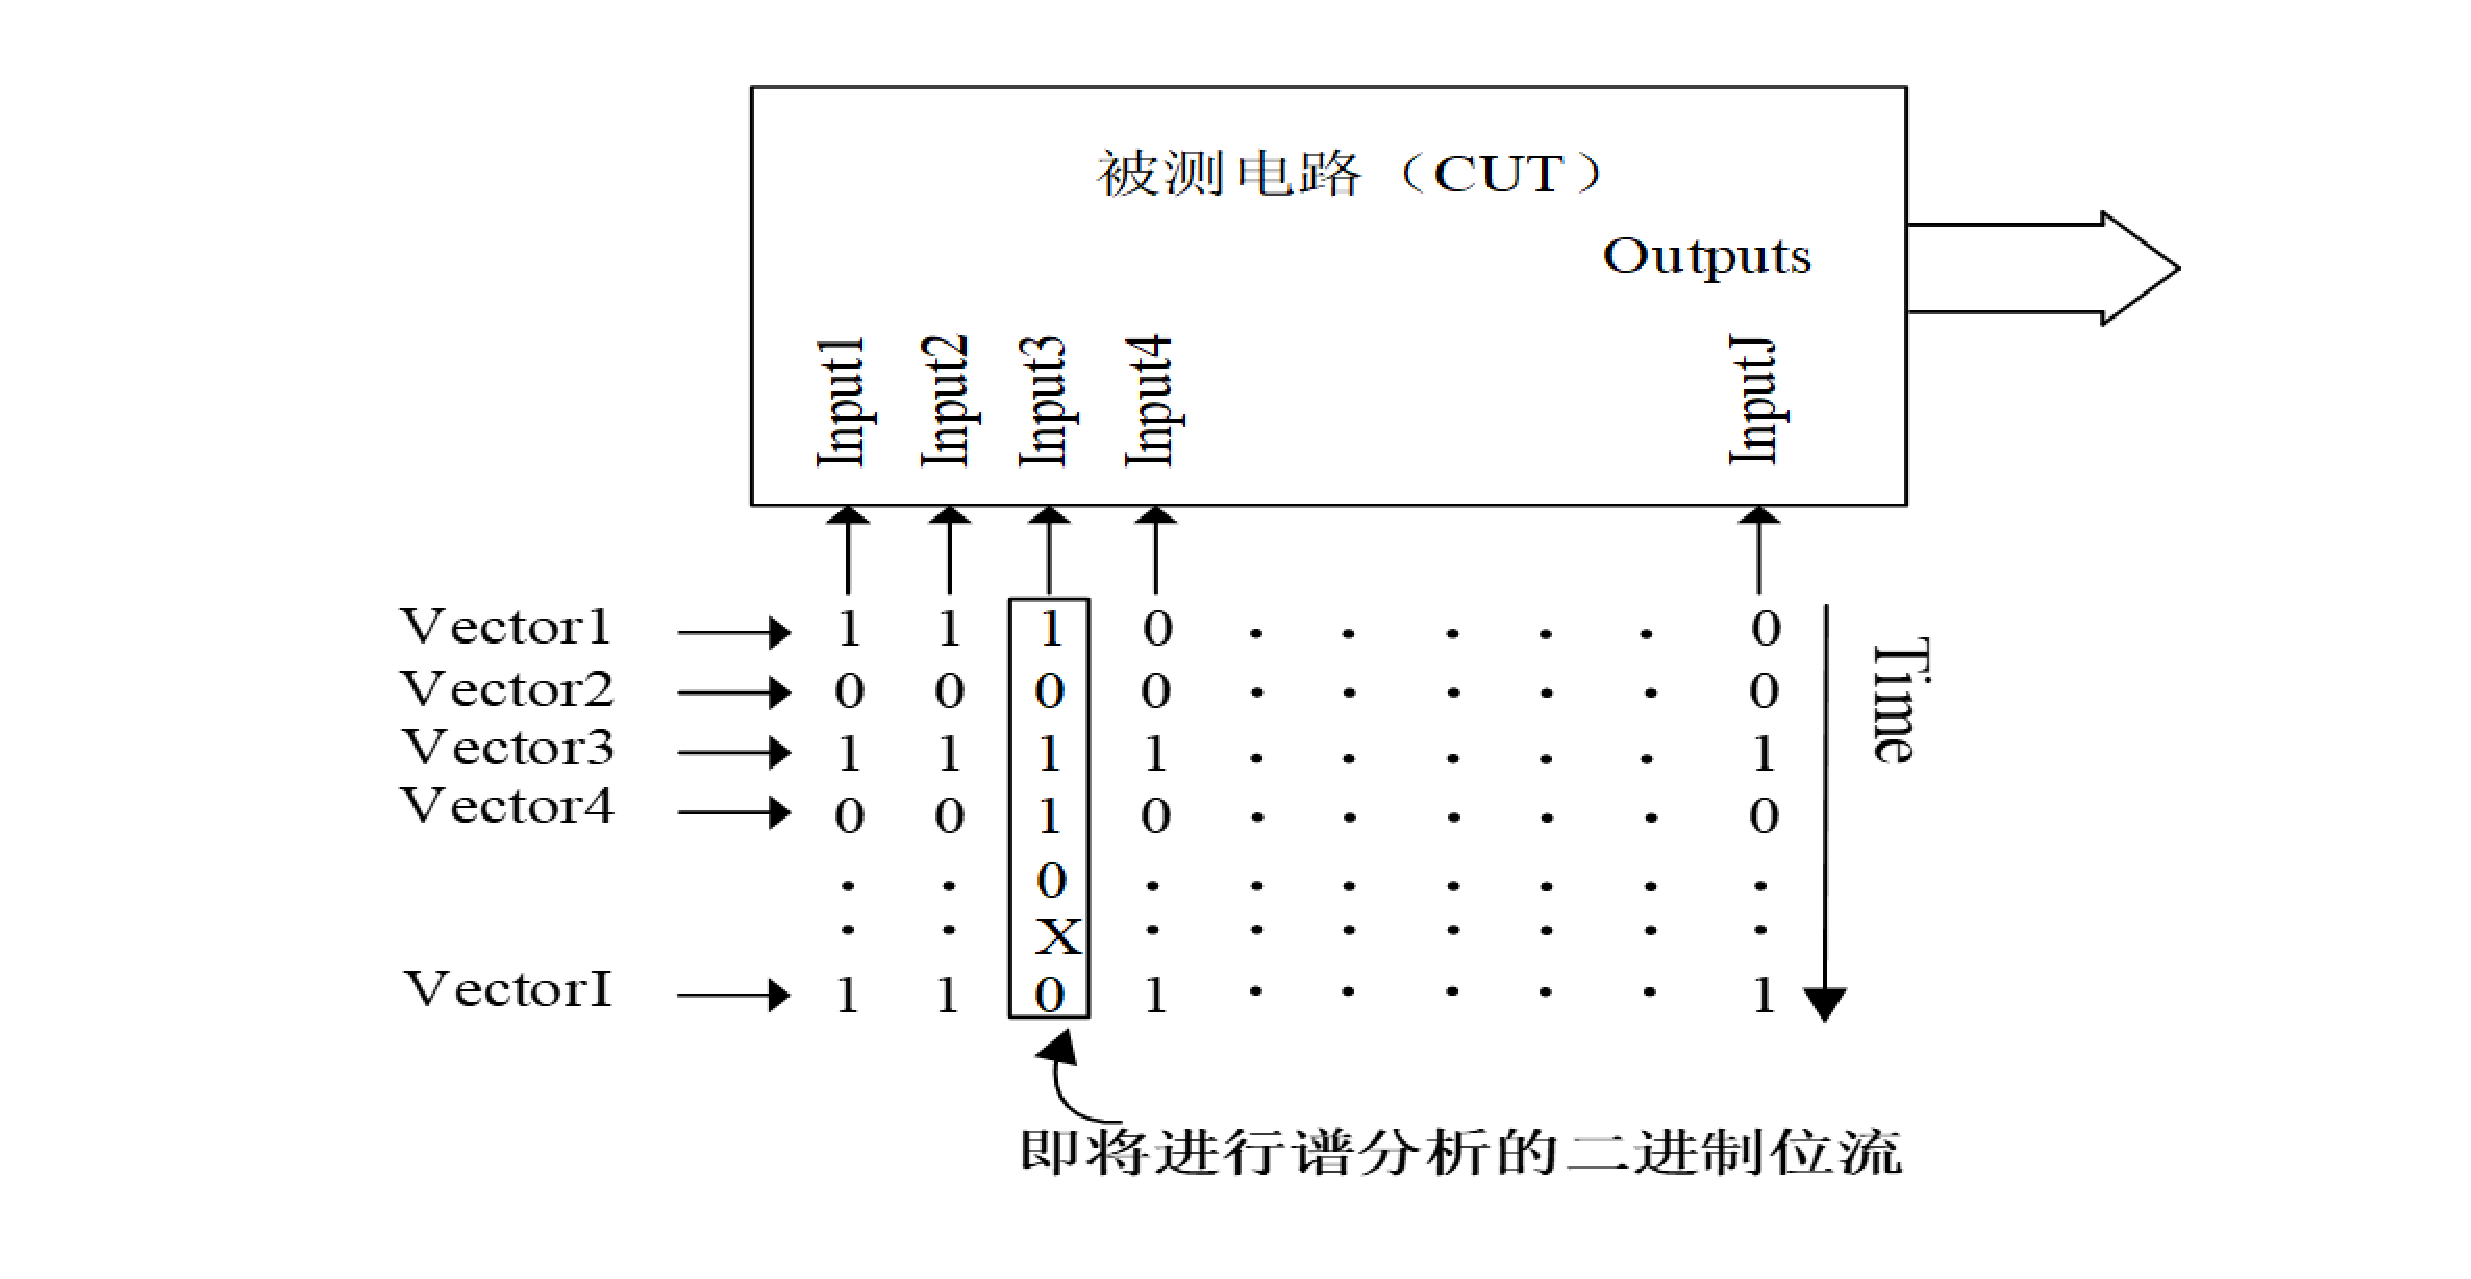
\includegraphics[height=10cm,width=16cm,angle=0,scale=1]{31.eps}
  \caption{测试立方和位流}\label{31}
     \end{figure}

向量分解的伪代码如下算法3.1所示,向量分解是为了提高残差集中0比特位的个数,对于单游程编码而言直接将无关位填充为0即可,拆分压缩技术对于双游程编码的压缩率提升较少,因为影响双游程编码压缩率的关键因素是跳变数,单纯地增加残分量集中的0也不一定会提高最终的压缩率。

\vspace{\baselineskip}
\begin{algorithm}[!h]
	\caption{向量分解}%算法标题
	\begin{algorithmic}%一行一个标行号
        \STATE $N:$ $Number$ $of$ $vectors$
		\STATE $M:$ $Number$ $of$ $inputs$
        \STATE $L:$ $LFSR$ $Matrix$
        \STATE $T[1:N, 1:M]:$ $Test$ $set$ $of$ $dimensions$ $N*M$
        \STATE $Initialization( T )$     // 预处理测试集合
		\FOR{$i=1$ to $M$}
        \STATE $p$ = $L*T[1:N, i]$      //测试集中每一列与位流相乘生成系数矩阵
        \STATE $k$ = $max( p )$         //在系数矩阵p中获取对应下表索引k
		\ENDFOR
		\STATE $Prominent$ = $L[k]$ //生成主分量
        \STATE $Residual$ = $T[1:N, i]$ $XOR$ $Prominent$   //获取残分量集
        \STATE $ProminentComponentSet.add(Prominent)$
        \STATE $ResidualComponentSet.add(Residual)$
        \STATE $Return ProminentComponentSet, ResidualComponentSet$  //返回所需数据
	\end{algorithmic}
\end{algorithm}

如矩阵3.1所示,将列向量(1, 0, 1, 1, 1, X, 0)谱分析后,向量转换为(1, -1, 1, 1, -1, 0, -1)。然后通过线性反馈移位寄存器变换,得到[2 -2 0 0 0 0 -2 5] 这个系数向量。系数向量中系数最大值对应的列向量就是所需的主分量,对应于上图的(1,-1,1,1,1,-1,-1),当系数向量中的最大值有多个时,可以任选其中的任一列作为所求的主分量。在本例中如果将原测试集的无关位填充为0,原列向量与主分量两两异或后最终所得的残差为(0,0,0,0,0,0,0),对于单游程编码,会产生极高的压缩率。若原测试集的列向量长度和线性反馈移位寄存器的矩阵行数不一致,则需要在位流尾部填充无关位或者截断基向量即可。

\begin{equation}
\left[
\begin{array}{ccccccc}
   1& -1& 1& 1& 1& 0& -1\\
\end{array}
\right]
=
\left[
\begin{array}{cccccccc}
    1&   1&   1&-1&   1&-1&-1&   1\\
    1&   1&-1&   1&   1&-1&   1&-1\\
    1&-1&-1&-1&   1&   1&   1&   1\\
    1&-1&   1&   1&-1&-1&   1&   1\\
    1&   1&-1&   1&-1&   1&-1&   1\\
    1&-1&   1&   1&   1&   1&-1&-1\\
    1&   1&   1&-1&-1&   1&   1&-1\\
\end{array}
\right]
\left[
\begin{array}{cccccccc}
   2& -2& 0& 0& 0& 0& -2& 5\\
\end{array}
\right]
\end{equation}

\section{预填充测试集}

\subsection{直接填充与策略填充}

如果采用编码压缩的方式对测试集进行压缩,一旦编码方式得以确定,无关位具体是填充0或者1也随之确定。直接填充就是将不确定位直接填充成为码字0 或者码字1,策略填充就是根据一定的策略进行填充,使得测试集在当前编码规则下的压缩率更高。填充完毕之后,当前的测试集中就不存在无关位,对于一个完全确定的测试集,可以选取合适的聚类算法来选取基向量,最后生成主分量集。本章依旧使用拆分压缩,当无关位填充之后,采取距离最大原则选取基向量生成主分量集。

在以往的研究过程中,并没有采取预填充的手段。对于主分量的选取,有的研究人员采用哈达码变换,有的采取最大相容类变换。通过哈达码变换可以取得较好的压缩增益,但是由于变换产生的列向量与原测试集无关,其获取的压缩率还有提升的空间。而采用最大相容类方式获取的压缩率并不高,由于使用KM算法或者贪婪算法结合关系矩阵法选取基向量,往往因为存在较多无关位,导致算法的时间复杂度过高。采用最大相容类方式确定的第一个基向量能与很多列向量相容,但继续往后选取,与其相容的会越来越少。基向量只能涵盖少数几列测试列向量,只有通过基向量之间两两异或扩展出的其他列向量与原测试中向量越相似,压缩效果才会越好。

\begin{equation}
A
=
\left[
\begin{array}{ccccccccc}
    X&   X&   1&X&   X&X&0&0&0\\
    0&   0&X&   X&   X&1&   1&X&X\\
   1&   0&0&   X&   X&X&   1&1&X\\
   1&   0&X&   X&   X&1&   1&X&X\\
   1&   1&X&   X&   X&X&   1&0&1\\
\end{array}
\right]
\end{equation}

通过一个例子来说明预填充方式的相关做法。上图给出原测试集,分别使用直接填充与策略填充的方式去除测试集中的无关位。下图1 是直接填充方式取得的测试集,采取的是0 填充的方式,如果采取1填充,则将无关为全部填充为1即可。

\begin{equation}
A
=
\left[
\begin{array}{ccccccccc}
    0&0&1&0&0&0&0&0&0\\
    0&0&0&0&0&1&1&0&0\\
    1&0&0&0&0&0&1&1&0\\
    1&0&0&0&0&1&1&0&0\\
    1&1&0&0&0&0&1&0&1\\
\end{array}
\right]
\end{equation}

如若采取策略填充,则需要选择一个默认的编码格式,本例采用FDR编码,直接将无关位填充为0即可,如上所示。如果采用双游程编码,要以原测试集的跳变数最少为原则对无关位进行填充,以EFDR编码为例,填充之后的测试集如下所示:

\begin{equation}
A
=
\left[
\begin{array}{ccccccccc}
   1&1&1&0&0&0&0&0&0\\
   0&0&0&0&0&1&1&1&1\\
   1&0&0&1&1&1&1&1&1\\
   1&0&1&1&1&1&1&1&1\\
   1&1&1&1&1&1&1&0&1\\
\end{array}
\right]
\end{equation}
游程编码不仅要保证跳变数最少,还需要权衡连续出现0或者1的个数,比如跳变数均为2,向量11XXXXXXXXXXXXX000总共有18位,此向量有多种填充方式,一种是将无关位全部填充0,一种是将无关位填充为1,本例应该采取全0方式填充,因为连续的确定位越多获得的压缩效果会越好。

\subsection{选取基向量}

基向量的选取方式至关重要,主分量集是由基向量集合确定的。若基向量集取自原测试集,由基向量集所产生的主分量集与原测试集中的向量相似度会更高,从而增加残差集中0的个数。在本文的第四章中使用聚类算法选取基向量,旨在使选出的基向量尽可能与原测试中的向量相似。为了更好地匹配原测试中已有的列向量,本文在原有的聚类算法上也做了相应的优化。

本章提取基向量的策略分三步进行,第一步随机从原测试集中选取一个列向量当作初始基向量$a$。第二步计算向量$a$与原测试集的每一列向量之间的欧几里得距离$dis$。$dis=\sqrt{((x_1-a_1)^2+(x_2-a_2)^2+....+(x_i-a_i)^2)}$,其中$x$为某一个基向量,$a$ 为原测试集中的某一个列向量,下标即为对应的位,取其中最大的$dis$对应的列向量作为新的基向量。第三步,根据当前确定的基向量求出全部初始基向量,后续步骤$dis$的计算方式为:
\begin{equation}\label{emd}
\centering
      dis=\min⁡(\sqrt{(x_1-a_1)^2+....+(x_i-a_i)^2},....,\sqrt{(y_1-a_1)^2+....+(y_i-a_i)^2)}
               \end{equation}

当有多列基向量时,$dis$为当前列向量与众多基向量两两之间求的欧几里得距离的最小值。对于不同的电路,选取基向量的个数也是不一样的,在本章中基向量选取的个数$X$计算的方式为$X\ge ceil(\log_2^n⁡)$,其中$n$代表当前测试集的行数,由于需要将$X$ 列基向量存储在被测电路中,因此$X$不能取过大,取的过大会浪费存储空间。$X$个列向量之间两两异或将产生$2^X-1$个列向量,主分量集就是由些列向量确定的。上文提及的哈达码矩阵,在拆分压缩中取得了较好的压缩率,$n$ 阶哈达码矩阵有$2^n$行、$2^n$ 列,其中$n$ 的值就是上述$x$ 的值,为了保证自变量一致,本文按照哈达码矩阵变换的规则选取基向量个数。

\section{实验结果与分析}

为了体现预填充方法的可行性,本文对 ISCAS’89\cite{71}中大部分电路进行了验证,包括S5378、S9234、S13207、S15850、S38417、S38584 等电路,本章将挑选其中部分电路做具体分析,计算出其在FDR、EFDR、Huffman 等编码方式下对应的压缩率,并与哈达码变换方法、极大相容类方法进行对比。

本文选取基向量的个数为$X\ge ceil(\log_2^n⁡)$ ,对于$X$列的基向量,两两异或最终可得$2^x-1$个列向量(集合$Y$)。从原测试集中选出每一列,然后将其与集合$Y$中的列向量一一对比,选取出最相似的一列并构造出一个新的集合,即主分量集。实验结果如下表\ref{mtabl1} 所示,首列为电路名称,第二列为当前电路的行数和列数,第三列是变换矩阵的个数,也就是$x$个列向量最终产生向量数的总和,第四列和第五列代表残差集所能达到的最小压缩率和最大压缩率。

\begin{table}[H]
\centering
\caption{随机矩阵与测试集变换结果}\label{mtabl1}
\begin{tabular}{p{2.2cm}p{2.7cm}<{\centering}p{3.3cm}<{\centering}p{2.7cm}<{\centering}p{2.7cm}<{\centering}}
\toprule
\textbf{电路名}&	\textbf{规模}&     \textbf{变换矩阵个数}&   \textbf{最小压缩率}&   \textbf{最大压缩率}\\
\midrule
s5378& (111,214)& 127& 59.64\%& 70.78\%\\
s9234& (159,247)& 255& 58.89\%& 70.12\%\\
s13207& (236,700)& 255& 72.17\%& 93.74\%\\
s15850& (126,611)& 127& 68.14\%& 83.30\%\\
s38417& (99,1664)& 127& 63.03\%& 75.74\%\\
s38584& (126,611)& 127& 68.14\%& 83.30\%\\
平均&        &      &   66.09\%& 78.05\%\\
\bottomrule
\end{tabular}
\end{table}

为了验证本实验是否对多种编码方式均适用,本文选取了FDR、EFDR、ALT-FDR以及Golomb等多种编码方式对变换拆分之后的残差集进行压缩,同时与使用哈达码变换达进行对比。本实验使用了直接填充与策略填充两种方式,直接填充1的效果相对较策略填充和全0填充效果差,策略填充和直接填充0作比较,直接填充0的效果甚至更好,因此为了最大化压缩率本文直接将无关位填充为0。

对于直接将无关位填充为0可以取得最佳的压缩率,猜想如下,第一:拆分压缩的目的是使得残差集中的0 更多,如果直接将无关位填充位0,可以增加残差集中0 的个数。第二:在选取基向量的过程中本文使用基向量之间两两距离最大的原则选取,增加了基向量异或之后所产生向量的多样性,从而获得了更多与原测试集中相似的向量,提高了压缩率。

下表\ref{mtabl2}-\ref{mtabl6}为本方法与哈达码变换以及最大相容类的压缩率对比情况,第一列代表电路名,第二列表示对电路直接使用编码压缩能取得的压缩率,第三列表示对原电路使用哈达码矩阵拆分压缩之后达到的压缩率,第四列为使用最大相容类提取主分量集所获取的压缩率,第五列为使用本方法所能达到的压缩率。以压缩率的提升为原则,本实验直接将无关位填充为0。

表\ref{mtabl2}为FDR编码下各电路的压缩率,电路s13207在不使用拆分压缩的方法下能取得80\%的压缩率,可以说明当前电路所包含的无关位较多。从表中数据可得,直接编码所获取的压缩率普遍较低,使用哈达码变换、最大相容类以及本章方法均可较为明显地提高压缩率。除了s38584 电路,使用预填充的方法所取得的压缩率均高于其他方法,因此取得了最高的平均压缩率。

\begin{table}[H]
\centering
\caption{FDR编码压缩率(\%)}\label{mtabl2}
\begin{tabular}{p{2.2cm}p{2.7cm}<{\centering}p{3.3cm}<{\centering}p{2.7cm}<{\centering}p{2.7cm}<{\centering}}
\toprule
\textbf{电路}&	\textbf{直接编码}& \textbf{哈达码变换}& \textbf{最大相容}& \textbf{本方法}\\
\midrule
s5378&	47.98&	67.51&	67.86&	68.43\\
s9234&	43.61&	66.19&	65.71&	66.39\\
s13207&	81.31&	89.65&	89.92&	91.69\\
s15850&	66.21&	80.66&	80.73&	81.88\\
s38417&	43.27&	72.44&	72.84&	73.04\\
s38584&	60.93&	75.99&	75.34&	75.09\\
平均&	57.22&	75.41&	75.35&	76.08\\
\bottomrule
\end{tabular}
\end{table}

以下是EFDR编码和VIHC编码所对应的压缩率,采用本方法所达到的平均压缩率比哈达码变换高0.79\%,比最大相容类高0.73\%,因此本方法不仅对单游程编码有效,也同样适用于其他编码方式。

\begin{table}[H]
\centering
\caption{EFDR编码压缩率(\%)}\label{mtabl3}
\begin{tabular}{p{2.2cm}p{2.7cm}<{\centering}p{3.3cm}<{\centering}p{2.7cm}<{\centering}p{2.7cm}<{\centering}}
\toprule
\textbf{电路}&	\textbf{直接编码}& \textbf{哈达码变换}& \textbf{最大相容}& \textbf{本方法}\\
\midrule
s5378&	53.67&	64.50&	64.52&	65.60\\
s9234&	48.66&	62.74&	62.62&	62.71\\
s13207&	82.49&	88.89&	88.03&	90.95\\
s15850&	68.66&	78.67&	78.83&	78.88\\
s38417&	62.02&	71.63&	71.76&	71.71\\
s38584&	64.28&	73.45&	72.37&	74.69\\
平均&	63.30&	73.30&	73.36&	74.09\\
\bottomrule
\end{tabular}
\end{table}

\begin{table}[H]
\centering
\caption{VIHC编码压缩率(\%)}\label{mtabl4}
\begin{tabular}{p{2.2cm}p{2.7cm}<{\centering}p{3.3cm}<{\centering}p{2.7cm}<{\centering}p{2.7cm}<{\centering}}
\toprule
\textbf{电路}&	\textbf{直接编码}& \textbf{哈达码变换}& \textbf{最大相容}& \textbf{本方法}\\
\midrule
s5378&	51.75&	69.63&	69.66&	70.78\\
s9234&	47.23&	69.58&	69.53&	70.12\\
s13207&	83.55&	92.20&	91.91&	93.74\\
s15850&	67.97&	82.96&	82.98&	83.30\\
s38417&	53.39&	74.79&	74.83&	75.74\\
s38584&	62.30&	78.11&	78.80&	79.50\\
平均&	61.03&	77.89&	77.83&	78.86\\
\bottomrule
\end{tabular}
\end{table}

\begin{table}[H]
\centering
\caption{RL-Huff编码压缩率(\%)}\label{mtabl5}
\begin{tabular}{p{2.2cm}p{2.7cm}<{\centering}p{3.3cm}<{\centering}p{2.7cm}<{\centering}p{2.7cm}<{\centering}}
\toprule
\textbf{电路}&	\textbf{直接编码}& \textbf{哈达码变换}& \textbf{最大相容}& \textbf{本方法}\\
\midrule
s5378&	52.58&	64.02&	64.14&	66.73\\
s9234&	47.26&	60.33&	60.16&	63.16\\
s13207&	82.49&	88.71&	88.81&	92.23\\
s15850&	67.35&	77.33&	77.99&	79.47\\
s38417&	63.32&	69.66&	69.64&	71.43\\
s38584&	62.40&	71.05&	72.28&	72.91\\
平均&	62.57&	71.85&	72.17&	74.32\\
\bottomrule
\end{tabular}
\end{table}

\begin{table}[H]
\centering
\caption{ALT-FDR编码压缩率(\%)}\label{mtabl6}
\begin{tabular}{p{2.2cm}p{2.7cm}<{\centering}p{3.3cm}<{\centering}p{2.7cm}<{\centering}p{2.7cm}<{\centering}}
\toprule
\textbf{电路}&	\textbf{直接编码}& \textbf{哈达码变换}& \textbf{最大相容}& \textbf{本方法}\\
\midrule
s5378&	49.95&	61.62&	62.02&	63.54\\
s9234&	44.96&	58.31&	58.16&	58.89\\
s13207&	80.23&	86.52&	86.61&	90.16\\
s15850&	65.83&	75.76&	75.89&	76.78\\
s38417&	60.55&	68.40&	67.51&	68.13\\
s38584&	61.13&	69.70&	71.83&	72.09\\
平均&	60.58&	70.06&	70.24&	71.60\\
\bottomrule
\end{tabular}
\end{table}

AFER和RL-Huff编码均是双游程编码,由上图可以得RL-Huff编码和ALT-FDR编码比哈达码变换所取得的压缩率平均高出2.47\%和1.54\%,比最大相容所取得的压缩率高2.15\%和1.36\%。

从表\ref{mtabl2}-\ref{mtabl6}中的结果可知,本方法与直接编码、哈达码变换以及最大相容类三种方法对比,均取得了较高的压缩率。

表\ref{mtabl7}中的数据为本方法与其他压缩方法在不同电路下获取的压缩增益,本方法的压缩率为使用FDR 编码所达,SVC 使用的是对称编码。L-EFDR 属于双游程编码,对EFDR 编码进行了改进,提高了压缩率。LHBE 方法先对确定位进行划分,再进行编码,降低了编码的比特数量。由实验结果可知,本方法的平均压缩率高达76.28\%,与其他压缩方法相比较均有提高。结果表明对无关位预填充,同时在选取基向量时,按照距离跨度最大的方式选取可以获取较高的压缩增益。从表中数据分析可知,不管使用何种压缩方法,s13207所取得的压缩率均是最高的,由此推断s13207电路中无关位会比较多。通过观察其测试集,也验证了这一推论。

\begin{table}[H]
\centering
\caption{本方法与其他压缩方法压缩率比较(\%)}\label{mtabl7}
\begin{tabular}{p{1.6cm}p{2.36cm}<{\centering}p{2.36cm}<{\centering}p{2.36cm}<{\centering}p{2.36cm}<{\centering}
p{2.36cm}<{\centering}}
\toprule
\textbf{电路名}&	\textbf{SVC\cite{72}	}& \textbf{I-EFDR\cite{73}}& \textbf{LHBE\cite{74}}& \textbf{CCPRL\cite{75}}& \textbf{本方法}\\
\midrule
s5378&	51.80&	55.10&	53.10&	61.08&	68.43\\
s9234& 	50.94& 	52.73& 	52.33& 	62.95&	66.39\\
s13207& 83.77& 	83.82& 	83.87& 	90.06& 	91.69\\
s15850& 69.98& 	71.05& 	70.78& 	76.32& 	80.88\\
s38417& 63.30& 	64.57& 	64.10& 	64.61& 	73.04\\
s38584& 66.26& 	66.70& 	66.60&	75.38& 	77.06\\
平均& 	64.34& 	68.01& 	65.13& 	71.73& 	76.28\\
\bottomrule
\end{tabular}
\end{table}

\section{小结}

为了降低电路的存储开销,提高数据压缩率,本章基于变换压缩的研究方法提出了一种预填充方法,此方法预先对测试集进行处理,去除原测试集中的无关位。此方法有直接填充与策略填充两种模式,对于拆分压缩直接将无关位填充为0效果最佳。其次,在基向量的选取过程中并不是一味随机选取,而是随机选取第一列,然后根据欧几里得距离依次确定其他的基向量,基向量两两之间差距的增大导致异或之后产生的列向量更加丰富,从而提高了压缩率。实验结果表明,使用本方法可以大大提高压缩率并减少了测试集的存储代价,节约测试时间成本。
